Το MIYearPicker Component αποτελείται από 2 κουμπιά και ένα πεδίο εισαγωγής όπως φαίνεται στο σχήμα \ref{layout:miyearpicker}. Όταν πατηθεί το κουμπί με το εικονίδιο ενός ημερολογίου η το πεδίο εισαγωγής, ανοίγει ένα μενού που επιτρέπει την επιλογή ενός έτους που υπάρχει για την επιλεγμένη κατηγορία ενώ όταν πατηθεί το κουμπί με εικονίδιο ένα "Χ" καθαρίζεται η επιλογή του έτους και εμφανίζονται τα συνολικά δεδομένα. Όταν εκτελεστεί μια ενέργεια από αυτό το Component, θα αλλάξει την διεύθυνση έτσι ώστε να αναλάβει το Dashboard Module την αλλαγή των δεδομένων όπως φαίνεται στον κώδικα \ref{code:miyearpicker_urlchanger}.
\begin{figure}[h]
  \centering
  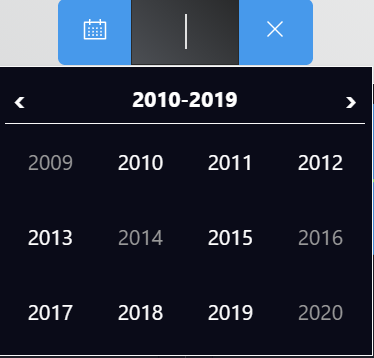
\includegraphics[width=35mm]{Chapters/5 - Architecture/Client/Images/miyearpicker.png}
  \caption{MIYearPicker Component}
  \label{layout:miyearpicker}
\end{figure}

\begin{figure}[h]
    \begin{TypeScriptcode}
yearSelected = (year: number) => {
  const activeView = this.props.rootState.dashboardState.activeView();
  const activeEntity = this.props.rootState.dashboardState.activeView().activeEntity;
  let role = null;
  if (activeView.entityType === EntityType.PERSON) {
    const _activeView = activeView as MovieInsightsPerPersonState;
    role = _activeView.activeRole;
  }
  this.props.history.push(AppUtils.|$\textbf{generateNavigationLink}$|(activeEntity.entity, role, year))
}
yearUnselected = () => {
  const activeEntity = this.props.rootState.dashboardState.activeView().activeEntity;
  if (activeEntity.entity) {
    this.props.history.push(AppUtils.|$\textbf{generateNavigationLink}$|(activeEntity.entity));
  } else {
    this.props.history.push(`/app`);
  }
}
    \end{TypeScriptcode}
    \caption{Αλγόριθμος αλλαγής διεύθυνσης απο το MIYearPicker Component.}
   \label{code:miyearpicker_urlchanger}
\end{figure}